\documentclass[14pt]{extreport}
\usepackage{amsfonts}
\usepackage[14pt]{extsizes}
\usepackage[left=3cm,right=2cm,
    top=2cm,bottom=2cm,bindingoffset=0cm]{geometry}
\renewcommand{\baselinestretch}{1.5}

\usepackage[utf8]{inputenc}
\usepackage[russian]{babel}
\usepackage{amsmath}
\usepackage{enumerate}
\usepackage{listings}
\usepackage{tocbibind}
\usepackage{appendix}
\usepackage{graphicx}
\usepackage{longtable}

\begin{document}
\pagenumbering{gobble} 

\begin{center}
МИНИСТЕРСТВО ОБРАЗОВАНИЯ И НАУКИ\\ РОССИЙСКОЙ ФЕДЕРАЦИИ\\[0.5cm]

МОСКОВСКИЙ ФИЗИКО-ТЕХНИЧЕСКИЙ ИНСТИТУТ\\
(государственный университет)\\[0.5cm]

ФАКУЛЬТЕТ ИННОВАЦИЙ И ВЫСОКИХ ТЕХНОЛОГИЙ\\
КАФЕДРА АНАЛИЗ ДАННЫХ\\[0.5cm]

(Специализация «Прикладные информационные технологии\\
в управлении и бизнесе»)\\[1.5cm]

{\bf ОТЫСКАНИЕ ОПТИМАЛЬНЫХ ПАРАМЕТРОВ}\\
{\bf В МОДЕЛЯХ СЛУЧАЙНЫХ ВЕБ-ГРАФОВ}\\[1.5cm]

Магистерская диссертация\\
студента 793 группы\\
Жернова Павла Владимировича\\[1.5cm]

Научный руководитель\\
Райгородский А.М., д.ф.-м.н.\\[3cm]


г. Москва\\
2013
\end{center}
\newpage
\pagenumbering{arabic} 
\setcounter{page}{2}
\tableofcontents
\newpage

\chapter{Введение}

Теория графов играет огромную роль, как в фундаментальной, так и в прикладной математике. Нас будет интересовать лишь одно направление, которое становится все более актуальным с каждым годом. Это графы, которые изучаются с вероятностной точки зрения. Случайные графы, которые описывают рост различных сетей, – социальных, биологических, транспортных – наиболее современны в этом направлении. В первую очередь, это связано, конечно же, с Интернетом.

\chapter{Модели случайных веб-графов}

Модели случайных веб-графов позволяют генерировать WWW-подобные графы, которые значительно меньше и проще, чем реальные WWW-графы, однако сохраняют определенные ключевые свойства структуры ребер веба. Такие искусственные графы можно рассматривать как экспериментальную платформу для получения новых подходов к поиску, индексации и т.д.
Вершины веб-графа соответствуют веб-страницам, а ребра – гиперссылкам между ними. Веб-графы довольно активно изучались на предмет различных числовых характеристик таких, как распределение, диаметр, число связных компонент, макроскопическая структура. Ниже приведем различные модели, призванные описывать реальные веб-графы.

Один из возможных теоретических подходов к модели веб-графа -- это математическая концепция случайного графа. Суть этого подхода заключается в том, что веб-граф развивается стохастически.
Было предпринято множество попыток смоделировать граф гиперссылок интернета как случайный граф. Наиболее простой и исторически первой является модель Эрдеша-Реньи.

\section{Модель Эрдеша-Реньи}  

Пусть $V_n = \{1,\dots,n\}$ -- множество вершин графа. Именно на них мы и будем строить наш случайный граф. Соединим любые две вершины $a$ и $b$ ребром с вероятностью $p \in [0, 1]$ независимо от всех остальных пар вершин. Другими словами, ребра в графе будут появляться в соответствии со схемой Бернулли, в которой вероятность успеха $p$ и $C_n^2$ испытаний (нас не интересуют кратные ребра, петли; граф неориентирован). Пусть $E$ -- случайное множество ребер, полученное в результате реализации такой схемы. Граф $G = (V_n, E)$ и есть случайный граф в модели Эрдеша-Реньи.

\section{Модели предпочтительного присоединения}

В 90-е годы XX века в своих работах Барабаши и Альберт описали некоторые статистики интернета -- веб-графа, вершинами которого являются страницы в интернете, а ребрами -- гиперссылки между ними. На самом деле, похожую структуру имеют также большинство других реальных сетей -- социальные, биологические, транспортные.

Основные результаты исследования Барабаши и Альберта состоят в следующем.
\begin{enumerate}

\item Веб-граф -- это <<разреженный>> граф. У него на $n$ вершинах всего $mn$ ребер, где $m \in \mathbb{Z}$ -- некоторая константа. Для сравнения, у полного графа на $n$ вершинах $C_n^2 \sim n^2$ ребер. 

\item Диаметр веб-графа очень мал (5-7, результат 1999 года). Это хорошо известное свойство любой социальной сети, которое принято называть <<мир тесен>>. Например, говорят, что любые 2 человека в мире <<знакомы через 5-6 рукопожатий>>. В интернете это свойство заключается в том, что кликая 5-7 раз по ссылкам можно перейти между любыми двумя страницами. (Если говорить более точно, то в интернете есть только что появившиеся сайты, которые могут быть не связаны с остальными сайтами. Поэтому правильнее сказать, что в интернете есть огромная компонента, диаметр которой мал). Итак, веб-граф обладает интересным свойством -- он разрежен, но при этом <<тесен>>.

\item Для веб-графа характерен степенной закон распределения степеней вершин. То есть, вероятность того, что вершина веб-графа имеет степень $d$ равна $cd^{-\gamma}$, где $\gamma = 2.1$. Интересно, что этот закон характерен для всех реальных сетей, но у каждой из них своя $\gamma$.
\end{enumerate}

Таким образом, описанная выше модель случайного графа Эрдеша-Реньи плохо описывает реальные веб-графы, поскольку графы, полученные в этой модели, не имеют степенного закона распределения степени вершины. 

Барабаши и Альберт предложили концепцию предпочтительного присоединения: граф строится с помощью случайного процесса, на каждом шаге которого добавляется новая вершина и фиксированное число ребер из новой вершины в уже существующие. При этом, вершины с большей степенью приобретают ребра с большей вероятностью, которая линейно зависит от их степени.

\section{Модель Боллобаша-Риордана}

Общая идея предпочтительного присоединения строго математически формулируется в модели Боллобаша-Риордана. Конструируется набор графов (марковская цепь) $G_m^n$, $n=1, 2, \dots,$ с $n$ вершинами и $mn$ ребрами, где $m \in \mathbb{Z}$ -- целое число. Сначала рассмотрим случай $m = 1$. Пусть граф $G_1^1$ -- граф, состоящий из одной вершины и одного ребра (петля). Граф $G_1^t$ получается из графа $G_1^{t-1}$ добавлением вершины t и ребра из вершины $t$ в вершину $i$, где $i$ выбирается из существующих в графе вершин случайно, согласно следующему распределению вероятностей:
$$  
P(i=s) =
\begin{cases}  
  d_{G_1^{t-1}}(s)/(2t-1),&\text{если $1 \le s \le t-1$,}\\
  1/(2t-1),&\text{если $s=t$,}\\
\end{cases}
$$  
где $d_{G_1^{t-1}(s)}$ -- степень вершины $s$ в графе $G_1^t$. 

Заметим, что распределение вероятностей задано корректно, поскольку:
$$
\sum_{i=1}^{t-1}\frac{d(i)}{2t-1} + \frac{1}{2t-1}=\frac{2t-2}{2t-1}+\frac{1}{2t-1}=1
$$

Случайный граф $G_1^n$ построен и он удовлетворяет принципу предпочтительного присоединения. Далее, граф $G_m^n$ строится из графа $G_1^{mn}$ объединением вершин $1, \dots, m$ в вершину $1$ нового графа, объединением вершин $m+1, \dots, 2m$ в вершину 2 нового графа и так далее. Замети, что можно аналогичным образом строить ориентированные графы: ребро между вершинами $i$ и $j$ идет из $i$ в $j$, если $i > j$.

\section{Модель Боллобаша-Риордана. Статическая модификация}

Существует также статическая модификация этой же модели. Статическая она потому, что в ней статическое описание случайности.
Итак, зафиксируем на оси абсцисс на плоскости $2n$ точек: $1, \dots, 2n$. Все точки разобьем на пары, каждую пару соединим дугой, которая лежит в верхней полуплоскости. Получится объект, который назовем {\it линейной хордовой диаграммой} ({\it lineared chord diagram или, сокращенно, LCD}). Заметим, что на $2n$ точках можно построить
$$
l_n = \frac{(2n)!}{2^nn!}
$$
различных LCD. По каждой LCD построим граф на $n$ вершинах и с $n$ ребрами. Алгоритм следующий: двигаемся оси абсцисс слева направо до тех пор, пока не обнаруживаем правый конец любой дуги. Пусть этот конец имеет номер $k_1$. Тогда множество ${1, \dots, k_1}$ делаем первой вершиной графа. Продолжаем двигаться от $k_1 + 1$ направо до следующего правого конца любой дуги $k_2$. Второй вершиной графа делаем набор ${k_1 + 1, \dots, k_2}$. Далее, аналогично. Всего правых концов $n$, поэтому мы получим граф на $n$ вершинах. Ребра в графе будем проводить по следующему правилу: две вершины соединяем ребром в том случае, если между соответствующими множествами точек есть дуга, при этом ребра ориентируются справа налево.

Далее, если считать LCD случайной, то есть полагать, что вероятность каждой LCD равна $1/l_n$, то возникают случайные графы. Можно доказать, что в определенном смысле такие графы очень похожи на $G_1^n$. Графы на $n$ вершинах и с $mn$ ребрами получаем так же, как и ранее.

\section{Модель Боллобаша-Риордана. Результаты}

Модель Боллобаша-Риордана хорошо отражает эмпирические свойства различных реальных графов. Во-первых, справедлива
\newtheorem{theorem}{Теорема}
\begin{theorem}
Для любого $k \ge 2$ и любого $\epsilon > 0$
$$
P\left((1-\epsilon)\frac{\log n}{\log \log n} \le diam G_k^n \le (1+\epsilon)\frac{\log n}{\log \log n}\right) \to 1, n \to \infty
$$
\end{theorem}
Это означает, что диаметр графа плотно сконцентрирован (по вероятности) около величины $\log n / \log \log n$, что согласуется с результатом 5-6 для 1999 года, потому что в интернете в 1999 году было $10^7$ вершин, значит
$$
\frac{\log 10^7}{\log \log 10^7} = \frac {7\log 10}{\log 7 + \log\log 10} \approx 6.
$$
Во-вторых, в 2001 году была доказана
\begin{theorem}
Для любого $k \ge 1$ и любого $d \le n^(\frac{1}{15})$
$$
M\left(\frac{|{i=1,\dots,n:deg_{G_k^n}i = d}|}{n}\right) \sim \frac{2k(k+1)}{(d+k+1)(d+k+2)(d+k+3)}.
$$
\end{theorem}

Поскольку $k$ -- константа, выражение в правой части имеет вид $const / d^3$, что и представляет из себя степенной закон.
У этой теоремы, однако, есть и неприятные моменты. Во-первых, из-за ограничения $d < n^(1/15)$ теорема не годится для практического применения. Во-вторых, степень $d$ в степенном законе в этой теореме равна 3, что расхождится с реальными графами, для которых $\gamma_{www}=2.1$. Это означает, что хоть модель Боллобаша-Риордана и отражает некоторые свойства интернета, она должна быть видоизменена, чтобы лучше соответствовать реальности.

\section{Модель Бакли-Остхуса}

Возможный подход к такому видоизменению -- это модель, независимо предложенная двумя группами исследователей. Они предложили расширить модель с помощью параметра, называемого {\it начальная аттрактивность вершины}. Это положительная константа, которая не зависит от степени. Позже Бакли и Остхус предложили явную конструкцию данной модели. Распределение степеней вершин в модели Бакли-Остхуса также подчиняется степенному закону, однако теперь варьируя значение параметра $a$ в определении модели можно изменять значение $\gamma$ результирущего графа.

Более строго, модель генерирует набор графов $H_{a, m}^n, n=1, 2,\dots,$ с $n$ вершинами и $mn$ ребрами, где $m \in \mathbb{Z}$ -- фиксированное число. Определение $H_{a, 1}^n$ повторяет определение $G_1^n$ с одним отличием, заключающимся в том, что вероятность нового ребра, добавляемого в $H_{a, 1}^n$ равна
$$  
P(i=s) =
\begin{cases}  
  \frac{d_{H_{a, 1}^{t-1}}(s)+a-1}{(a+1)t-1},&\text{если $1 \le s \le t-1$,}\\
  \frac{a}{(a+1)t-1},&\text{если $s=t$,}\\
\end{cases}
$$  
Граф $H_{a, m}^n$ получается из графа $H_{a, 1}^{mn}$ так же, как и $G_m^n$ получается из $G_1^{mn}$. Заметим, что при $a=1$ мы получаем изначальную модель Боллобаша-Риордана $G_m^n$. Для целых $a$ Бакли и Остхус доказали, что распределение степеней вершин случайного графа в модели соответствует степенному закону с $\gamma = 2 + a$.
 
\section{Модель Боллобаша-Боргса-Риордана-Чайеса}

В данной модели строится ориентированный граф итеративно, на каждом шаге добавляется одно ребро. На каждом шаге также может быть добавлена одна вершина. Для простоты будем считать, что в графе могут присутствовать множественные ребра и петли.

Более строго, пусть $\alpha, \beta, \gamma, \delta_{in}$ и $\delta_{out}$ -- неотрицательные действительные числа такие, что $\alpha + \beta + \gamma = 1$. Пусть $G_0$ -- фиксированный начальный ориентированный граф, например, одна вершина без ребер, и пусть $t_0$ -- это число ребер в графе $G_0$. (В зависимости от параметров может понадобиться положить $t_0 \ge 1$, чтобы на первых шагах процесс имел смысл). Положим $G(t_0) = G_0$, то есть в момент времени $t$ граф $G(t)$ имеет ровно $t$ ребер и случайное число $n(t)$ вершин.

Для упрощения описания модели, условимся под фразой <<{\it выбрать} вершину $v$ графа $G(t)$ {\it в соответствии} с $d_{out} + \delta_{out}$>> понимать, что вершина $v$ выбирается таким образом, что $Pr(v=v_i)$ пропорциональна $d_{out}(v_i) + \delta_{out}$, то есть таким образом, что $Pr(v=v_i)=(d_{out}(v_i) + \delta_{out})/(t  + \delta_{out}n(t))$. Аналогично, под фразой <<{\it выбрать} $v$ {\it в соответствии с} $d_{in} + \delta_{in}$>> будем понимать, что вершина $v$ выбирается таким образом, что $Pr(v=v_i)=(d_{in}(v_i) + \delta_{in})/(t  + \delta_{in}n(t))$. Здесь $d_{out}(v_i)$ и $d_{in}(v_i)$ -- исходящая и входящая степени вершины $v_i$ в графе $G(t)$.

Для $t \ge t_0$ граф $G(t+1)$ строится из графа $G(t)$ по следующим правилам:
\begin{enumerate}
\item С вероятностью $\alpha$ добавляется новая вершина $v$ вместе с ребром из $v$ в существующую вершину $w$, где $w$ выбирается в соответствии с $d_{in} + \delta_{in}$.
\item С вероятностью $\beta$ добавляется ребро из существующей вершины $v$ в существующую вершину $w$, где $v$ и $w$ выбираются независимо, $v$ в соответствии с $d_{out} + \delta_{out}$, а $w$ в соответствии с $d_{in} + \delta_{in}$.
\item С вероятностью $\gamma$ добавляется новая вершина $w$ и ребро из существующей вершины $v$ в вершину $w$, где $v$ выбирается в соответствии с $d_{out} + \delta_{out}$.
\end{enumerate}

Понятно, что вероятности $\alpha$, $\beta$ и $\gamma$ должны в сумме давать единицу. Чтобы граф не был тривиальным, необходимо также положить $\alpha + \gamma$ > 0. Заметим также, что для веб-графа естественно взять $\delta_{out} = 0$, потому что вершины, добавляемые в третьем случае соответствуют веб-страницам, которые просто предоставляют некий контент. Такие страницы никогда не изменяются, они <<рождаются>> без исходящих ссылок и сохраняют это свойство. Вершины, добавляемые в первом случае соответствуют обычным страницам, ссылки на которые могут быть добавлены позже. Также, чисто математически кажется естественным положить и $\delta_{in} = 0$ на ряду с $\delta_{out} = 0$, однако это приводит к модели, в которой каждая страница не из $G_0$ не будет иметь либо входящих ссылок, либо исходящих, что довольно нереалистично и неинтересно! Ненулевое значение $\delta_{in}$ говорит о том, что вершина не является частью веба до тех пор, пока на нее не появятся ссылки, обычно с одного из крупных поисковых сервисов. Эти ссылки с поисковых сервисов естественно рассматривать отдельно от графа, поскольку они имеют другую природу. По той же причине $\delta_{in}$ не обязательно должно быть целым числом. Параметр $\delta_{out}$ все же включается в модель для симметрии и для большей общности.

Модель допускает наличие в графе петель и кратных ребер; нет оснований для исключения их из графа. Более того, их число оказывается небольшим, поэтому они незначительно влияют на численные эксперименты. 

\section{Модель копирования}

Эта модель возникла практически в одно время с моделью Барабаши-Альберт. Ее авторами являются Р. Кумар, П. Рагхаван, С. Раджагопалан, Д. Сивакумар, А. Томкинс и Э. Упфал.

Зафиксируем $\alpha \in (0,1)$ и $d \ge 1, d \in \mathbb{N}$. Граф будем строить итеративно, в качества начального графа $G_0$ возьмем $d$-регулярный граф (граф, у которого степень каждой вершины равна $d$). Пусть граф с номером $t$ уже построен -- это граф $G_t = (V_t, E_t)$, где $V_t = \{u_1, \dots, u_s\}$, а $s$ отличается от $t$ на число вершин начального графа $G_0$, то есть на $const(d)$. Добавим теперь к графу $G_t$ новую вершину $u_{s+1}$ и $d$ ребер, выходящих из нее. Сделаем это следующим образом: сначала выберем случайную вершину $p \in V_t$ (все вершины $V_t$ равновероятны), затем построим $d$ ребер из $u_{s+1}$ в $V_t$ за $d$ шагов. На каждом шаге с вероятностью $\alpha$ проводим ребро из $u_{s+1}$ в случайную вершину из $V_t$ (все вершины $V_t$ равновероятны), а с вероятностью $1-\alpha$ проводим ребро из $u_{s+1}$ в i-го соседа вершины $p$, который всегда найдется, потому что у каждой вершины не менее $d$ соседей. 

\chapter{Экспериментальная часть}

Предметом исследования в данной работе является модель Боллобаша-Боргса-Риордана-Чайеса.

\section{Постановка эксперимента}

Рассмотрим степенное распределение степеней вершин графа
$$
P = c d^{-\xi},
$$
где $d$ -- степень вершины графа, $P$ -- вероятность встретить вершину степени $d$ в данном графе (то есть отношение количества вершин степени $d$ к общему количеству вершни в графе), $c$ и $\xi$ -- некие константы.

Будем считать, что величина $\xi$ является характеристикой графа, по которой можно сравнить несколько графов, то есть эта величина выступает в качестве метрики при сравнении графов. Чем меньше модуль разности между этими величинами у различных графов, тем больше эти графы будем считать похожими друг на друга.

Целью эксперимента является подбор оптимальных параметров $\alpha$, $\beta$, $\gamma$, $\delta_{in}$ и $\delta_{out}$ модели Боллобаша-Боргса-Риордана-Чайеса, при которых величина $\xi$ для модельного графа окажется максимально близкой к величине $\xi$ для реального веб-графа.

Параметр $\gamma = 1 - \alpha - \beta$, а параметр $\delta_{out} = 0$. Поэтому достаточно перебрать значения параметров $\alpha$, $\beta$ и $\delta_{in}$. Значения $\alpha$ и $\beta$ могут быть от $0$ до $1$ включительно, однако исключим вырожденные случаи и будем рассматривать значения $\alpha$ и $\beta$ из множества $\left\{0.1, 0.2, 0.3, 0.4, 0.5, 0.6, 0.7, 0.8, 0.9\right\}$, причём $\alpha + \beta < 1$. Значения параметра $\delta_{in}$ рассмотрим из множества $\left\{10, 20, 30, 40, 50\right\}$.

В качестве реального веб-графа будет рассматривать срез Интернет-графа за 2005 год, сделанный роботом ведущей российской компании, занимающейся поиском в сети Интернет.

\section{Результат эксперимента для реального графа}

В ходе эксперимента для реального графа получилось значение $\xi = 1.28909$.

Если полученное распределение отобразить на графике с логарифмическими шкалами по обеим осям, отложив степени вершин $d$ по горизонтальной оси и вероятности $P$ по вертикальной оси, то вместе с апроксиммирующей прямой методом наименьших квадратов получаем такой результат:

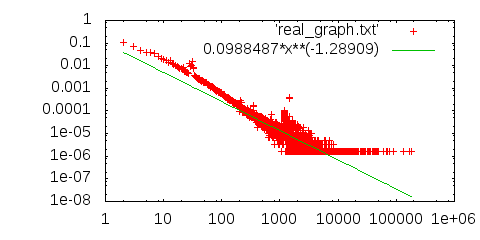
\includegraphics[width=160mm]{code/real_graph.png}

\section{Результат эксперимента для модельного графа}

Для каждого набора параметров строим модельный граф с временем $t = 100000$ три раза, а потом вычисляем математическое ожидание и дисперсию величины $\xi$ и ищем те значения параметров, при которых среднее значение $\xi$ модельного графа почти совпадёт с значением $\xi$ для реального графа.

В ходе эксперимента были получены следующие результаты:

\begin{center}
\begin{longtable}{|p{1cm}|p{1cm}|p{1cm}|p{1cm}|p{1cm}|p{8cm}|} \hline
$\alpha$ & $\beta$ & $\gamma$ & $\delta_{in}$ & $\delta_{out}$ & $\xi$ \\ \hline
\endfirsthead
\hline
$\alpha$ & $\beta$ & $\gamma$ & $\delta_{in}$ & $\delta_{out}$ & $\xi$ \\ \hline
\endhead
\endfoot
\endlastfoot
$0.1$ & $0.1$ & $0.8$ & $10$ & $0$ & $0.932771 \pm 0.00728888$ \\ \hline
$0.1$ & $0.1$ & $0.8$ & $20$ & $0$ & $0.974909 \pm 0.000788533$ \\ \hline
$0.1$ & $0.1$ & $0.8$ & $30$ & $0$ & $0.969449 \pm 0.000961652$ \\ \hline
$0.1$ & $0.1$ & $0.8$ & $40$ & $0$ & $0.961931 \pm 0.000463594$ \\ \hline
$0.1$ & $0.1$ & $0.8$ & $50$ & $0$ & $0.931287 \pm 0.000423722$ \\ \hline
$0.1$ & $0.2$ & $0.7$ & $10$ & $0$ & $0.99747 \pm 0.000663344$ \\ \hline
$0.1$ & $0.2$ & $0.7$ & $20$ & $0$ & $0.97063 \pm 0.00198001$ \\ \hline
$0.1$ & $0.2$ & $0.7$ & $30$ & $0$ & $0.94963 \pm 0.00000200138$ \\ \hline
$0.1$ & $0.2$ & $0.7$ & $40$ & $0$ & $1.08471 \pm 0.00390443$ \\ \hline
$0.1$ & $0.2$ & $0.7$ & $50$ & $0$ & $1.02931 \pm 0.000443945$ \\ \hline
$0.1$ & $0.3$ & $0.6$ & $10$ & $0$ & $1.01148 \pm 0.00112183$ \\ \hline
$0.1$ & $0.3$ & $0.6$ & $20$ & $0$ & $0.994045 \pm 0.000407881$ \\ \hline
$0.1$ & $0.3$ & $0.6$ & $30$ & $0$ & $1.07286 \pm 0.000944741$ \\ \hline
$0.1$ & $0.3$ & $0.6$ & $40$ & $0$ & $1.00004 \pm 0.00199681$ \\ \hline
$0.1$ & $0.3$ & $0.6$ & $50$ & $0$ & $0.975628 \pm 0.00530568$ \\ \hline
$0.1$ & $0.4$ & $0.5$ & $10$ & $0$ & $1.06259 \pm 0.0029934$ \\ \hline
$0.1$ & $0.4$ & $0.5$ & $20$ & $0$ & $1.06301 \pm 0.00134939$ \\ \hline
$0.1$ & $0.4$ & $0.5$ & $30$ & $0$ & $1.02225 \pm 0.000126111$ \\ \hline
$0.1$ & $0.4$ & $0.5$ & $40$ & $0$ & $1.09805 \pm 0.000911361$ \\ \hline
$0.1$ & $0.4$ & $0.5$ & $50$ & $0$ & $1.06724 \pm 0.000594735$ \\ \hline
$0.1$ & $0.5$ & $0.4$ & $10$ & $0$ & $1.10449 \pm 0.0000661492$ \\ \hline
$0.1$ & $0.5$ & $0.4$ & $20$ & $0$ & $1.09398 \pm 0.0000102478$ \\ \hline
$0.1$ & $0.5$ & $0.4$ & $30$ & $0$ & $1.10271 \pm 0.000873227$ \\ \hline
$0.1$ & $0.5$ & $0.4$ & $40$ & $0$ & $1.03951 \pm 0.000933735$ \\ \hline
$0.1$ & $0.5$ & $0.4$ & $50$ & $0$ & $1.08029 \pm 0.00161058$ \\ \hline
$0.1$ & $0.6$ & $0.3$ & $10$ & $0$ & $1.20919 \pm 0.000494145$ \\ \hline
$0.1$ & $0.6$ & $0.3$ & $20$ & $0$ & $1.14218 \pm 0.000446993$ \\ \hline
$0.1$ & $0.6$ & $0.3$ & $30$ & $0$ & $1.1227 \pm 0.00196923$ \\ \hline
$0.1$ & $0.6$ & $0.3$ & $40$ & $0$ & $1.14014 \pm 0.00798361$ \\ \hline
$0.1$ & $0.6$ & $0.3$ & $50$ & $0$ & $1.13292 \pm 0.00204208$ \\ \hline
$0.1$ & $0.7$ & $0.2$ & $10$ & $0$ & $1.23367 \pm 0.00132783$ \\ \hline
$0.1$ & $0.7$ & $0.2$ & $20$ & $0$ & $1.18782 \pm 0.00428949$ \\ \hline
$0.1$ & $0.7$ & $0.2$ & $30$ & $0$ & $1.27585 \pm 0.00275136$ \\ \hline
$0.1$ & $0.7$ & $0.2$ & $40$ & $0$ & $1.22912 \pm 0.00039264$ \\ \hline
$0.1$ & $0.7$ & $0.2$ & $50$ & $0$ & $1.17065 \pm 0.00339632$ \\ \hline
$0.1$ & $0.8$ & $0.1$ & $10$ & $0$ & $1.26342 \pm 0.00249616$ \\ \hline
$0.1$ & $0.8$ & $0.1$ & $20$ & $0$ & $1.29528 \pm 0.00196035$ \\ \hline
$0.1$ & $0.8$ & $0.1$ & $30$ & $0$ & $1.25078 \pm 0.00301471$ \\ \hline
$0.1$ & $0.8$ & $0.1$ & $40$ & $0$ & $1.23568 \pm 0.00087426$ \\ \hline
$0.1$ & $0.8$ & $0.1$ & $50$ & $0$ & $1.25477 \pm 0.000962454$ \\ \hline
$0.2$ & $0.1$ & $0.7$ & $10$ & $0$ & $1.23841 \pm 0.000770949$ \\ \hline
$0.2$ & $0.1$ & $0.7$ & $20$ & $0$ & $1.19279 \pm 0.000768557$ \\ \hline
$0.2$ & $0.1$ & $0.7$ & $30$ & $0$ & $1.189 \pm 0.000427635$ \\ \hline
$0.2$ & $0.1$ & $0.7$ & $40$ & $0$ & $1.17462 \pm 0.000312942$ \\ \hline
$0.2$ & $0.1$ & $0.7$ & $50$ & $0$ & $1.22531 \pm 0.00285168$ \\ \hline
$0.2$ & $0.2$ & $0.6$ & $10$ & $0$ & $1.27213 \pm 0.00168208$ \\ \hline
$0.2$ & $0.2$ & $0.6$ & $20$ & $0$ & $1.26298 \pm 0.0000707486$ \\ \hline
$0.2$ & $0.2$ & $0.6$ & $30$ & $0$ & $1.2835 \pm 0.00280229$ \\ \hline
$0.2$ & $0.2$ & $0.6$ & $40$ & $0$ & $1.26348 \pm 0.000511625$ \\ \hline
$0.2$ & $0.2$ & $0.6$ & $50$ & $0$ & $1.20518 \pm 0.00345746$ \\ \hline
$0.2$ & $0.3$ & $0.5$ & $10$ & $0$ & $1.23412 \pm 0.00104592$ \\ \hline
$0.2$ & $0.3$ & $0.5$ & $20$ & $0$ & $1.2875 \pm 0.000527015$ \\ \hline
$0.2$ & $0.3$ & $0.5$ & $30$ & $0$ & $1.28566 \pm 0.00430134$ \\ \hline
$0.2$ & $0.3$ & $0.5$ & $40$ & $0$ & $1.22661 \pm 0.000687818$ \\ \hline
$0.2$ & $0.3$ & $0.5$ & $50$ & $0$ & $1.28648 \pm 0.000353701$ \\ \hline
$0.2$ & $0.4$ & $0.4$ & $10$ & $0$ & $1.30134 \pm 0.000357783$ \\ \hline
$0.2$ & $0.4$ & $0.4$ & $20$ & $0$ & $1.29683 \pm 0.000250697$ \\ \hline
$0.2$ & $0.4$ & $0.4$ & $30$ & $0$ & $1.33242 \pm 0.00190293$ \\ \hline
$0.2$ & $0.4$ & $0.4$ & $40$ & $0$ & $1.30397 \pm 0.00000382383$ \\ \hline
$0.2$ & $0.4$ & $0.4$ & $50$ & $0$ & $1.28801 \pm 0.00389082$ \\ \hline
$0.2$ & $0.5$ & $0.3$ & $10$ & $0$ & $1.36286 \pm 0.000763779$ \\ \hline
$0.2$ & $0.5$ & $0.3$ & $20$ & $0$ & $1.30001 \pm 0.00136646$ \\ \hline
$0.2$ & $0.5$ & $0.3$ & $30$ & $0$ & $1.33997 \pm 0.00108664$ \\ \hline
$0.2$ & $0.5$ & $0.3$ & $40$ & $0$ & $1.37349 \pm 0.0039013$ \\ \hline
$0.2$ & $0.5$ & $0.3$ & $50$ & $0$ & $1.33394 \pm 0.000192949$ \\ \hline
$0.2$ & $0.6$ & $0.2$ & $10$ & $0$ & $1.4149 \pm 0.00720377$ \\ \hline
$0.2$ & $0.6$ & $0.2$ & $20$ & $0$ & $1.42447 \pm 0.00134053$ \\ \hline
$0.2$ & $0.6$ & $0.2$ & $30$ & $0$ & $1.38158 \pm 0.000679881$ \\ \hline
$0.2$ & $0.6$ & $0.2$ & $40$ & $0$ & $1.39088 \pm 0.000561193$ \\ \hline
$0.2$ & $0.6$ & $0.2$ & $50$ & $0$ & $1.34371 \pm 0.000489887$ \\ \hline
$0.2$ & $0.7$ & $0.1$ & $10$ & $0$ & $1.43066 \pm 0.000642419$ \\ \hline
$0.2$ & $0.7$ & $0.1$ & $20$ & $0$ & $1.46199 \pm 0.0000889685$ \\ \hline
$0.2$ & $0.7$ & $0.1$ & $30$ & $0$ & $1.46693 \pm 0.00109336$ \\ \hline
$0.2$ & $0.7$ & $0.1$ & $40$ & $0$ & $1.44535 \pm 0.00547142$ \\ \hline
$0.2$ & $0.7$ & $0.1$ & $50$ & $0$ & $1.47933 \pm 0.00261129$ \\ \hline
$0.3$ & $0.1$ & $0.6$ & $10$ & $0$ & $1.44605 \pm 0.00110126$ \\ \hline
$0.3$ & $0.1$ & $0.6$ & $20$ & $0$ & $1.49866 \pm 0.00207915$ \\ \hline
$0.3$ & $0.1$ & $0.6$ & $30$ & $0$ & $1.4928 \pm 0.00290065$ \\ \hline
$0.3$ & $0.1$ & $0.6$ & $40$ & $0$ & $1.47628 \pm 0.00233522$ \\ \hline
$0.3$ & $0.1$ & $0.6$ & $50$ & $0$ & $1.47639 \pm 0.00105536$ \\ \hline
$0.3$ & $0.2$ & $0.5$ & $10$ & $0$ & $1.5047 \pm 0.00204238$ \\ \hline
$0.3$ & $0.2$ & $0.5$ & $20$ & $0$ & $1.51964 \pm 0.000521645$ \\ \hline
$0.3$ & $0.2$ & $0.5$ & $30$ & $0$ & $1.48895 \pm 0.00135505$ \\ \hline
$0.3$ & $0.2$ & $0.5$ & $40$ & $0$ & $1.53566 \pm 0.000545929$ \\ \hline
$0.3$ & $0.2$ & $0.5$ & $50$ & $0$ & $1.47804 \pm 0.00143119$ \\ \hline
$0.3$ & $0.3$ & $0.4$ & $10$ & $0$ & $1.52457 \pm 0.000237678$ \\ \hline
$0.3$ & $0.3$ & $0.4$ & $20$ & $0$ & $1.52941 \pm 0.000652224$ \\ \hline
$0.3$ & $0.3$ & $0.4$ & $30$ & $0$ & $1.51453 \pm 0.00176311$ \\ \hline
$0.3$ & $0.3$ & $0.4$ & $40$ & $0$ & $1.55945 \pm 0.0000687918$ \\ \hline
$0.3$ & $0.3$ & $0.4$ & $50$ & $0$ & $1.53562 \pm 0.00641355$ \\ \hline
$0.3$ & $0.4$ & $0.3$ & $10$ & $0$ & $1.60746 \pm 0.000783873$ \\ \hline
$0.3$ & $0.4$ & $0.3$ & $20$ & $0$ & $1.53671 \pm 0.00185931$ \\ \hline
$0.3$ & $0.4$ & $0.3$ & $30$ & $0$ & $1.59394 \pm 0.00932542$ \\ \hline
$0.3$ & $0.4$ & $0.3$ & $40$ & $0$ & $1.56606 \pm 0.000836987$ \\ \hline
$0.3$ & $0.4$ & $0.3$ & $50$ & $0$ & $1.56114 \pm 0.00178809$ \\ \hline
$0.3$ & $0.5$ & $0.2$ & $10$ & $0$ & $1.65333 \pm 0.00334823$ \\ \hline
$0.3$ & $0.5$ & $0.2$ & $20$ & $0$ & $1.63995 \pm 0.0030323$ \\ \hline
$0.3$ & $0.5$ & $0.2$ & $30$ & $0$ & $1.67205 \pm 0.00117298$ \\ \hline
$0.3$ & $0.5$ & $0.2$ & $40$ & $0$ & $1.65376 \pm 0.000025201$ \\ \hline
$0.3$ & $0.5$ & $0.2$ & $50$ & $0$ & $1.608 \pm 0.000610703$ \\ \hline
$0.3$ & $0.6$ & $0.1$ & $10$ & $0$ & $1.71611 \pm 0.000653836$ \\ \hline
$0.3$ & $0.6$ & $0.1$ & $20$ & $0$ & $1.67483 \pm 0.00165382$ \\ \hline
$0.3$ & $0.6$ & $0.1$ & $30$ & $0$ & $1.67222 \pm 0.00446685$ \\ \hline
$0.3$ & $0.6$ & $0.1$ & $40$ & $0$ & $1.67199 \pm 0.000164499$ \\ \hline
$0.3$ & $0.6$ & $0.1$ & $50$ & $0$ & $1.70552 \pm 0.000339063$ \\ \hline
$0.4$ & $0.1$ & $0.5$ & $10$ & $0$ & $1.85665 \pm 0.000804998$ \\ \hline
$0.4$ & $0.1$ & $0.5$ & $20$ & $0$ & $1.82345 \pm 0.00610725$ \\ \hline
$0.4$ & $0.1$ & $0.5$ & $30$ & $0$ & $1.78459 \pm 0.000654807$ \\ \hline
$0.4$ & $0.1$ & $0.5$ & $40$ & $0$ & $1.81684 \pm 0.00544487$ \\ \hline
$0.4$ & $0.1$ & $0.5$ & $50$ & $0$ & $1.82816 \pm 0.00448046$ \\ \hline
$0.4$ & $0.2$ & $0.4$ & $10$ & $0$ & $1.84631 \pm 0.00114318$ \\ \hline
$0.4$ & $0.2$ & $0.4$ & $20$ & $0$ & $1.84171 \pm 0.00335591$ \\ \hline
$0.4$ & $0.2$ & $0.4$ & $30$ & $0$ & $1.83696 \pm 0.000794708$ \\ \hline
$0.4$ & $0.2$ & $0.4$ & $40$ & $0$ & $1.80721 \pm 0.000486551$ \\ \hline
$0.4$ & $0.2$ & $0.4$ & $50$ & $0$ & $1.81096 \pm 0.00400177$ \\ \hline
$0.4$ & $0.3$ & $0.3$ & $10$ & $0$ & $1.88461 \pm 0.00351277$ \\ \hline
$0.4$ & $0.3$ & $0.3$ & $20$ & $0$ & $1.91742 \pm 0.00201697$ \\ \hline
$0.4$ & $0.3$ & $0.3$ & $30$ & $0$ & $1.86504 \pm 0.00102953$ \\ \hline
$0.4$ & $0.3$ & $0.3$ & $40$ & $0$ & $1.86436 \pm 0.000598827$ \\ \hline
$0.4$ & $0.3$ & $0.3$ & $50$ & $0$ & $1.87625 \pm 0.000134616$ \\ \hline
$0.4$ & $0.4$ & $0.2$ & $10$ & $0$ & $1.9842 \pm 0.0052373$ \\ \hline
$0.4$ & $0.4$ & $0.2$ & $20$ & $0$ & $1.93133 \pm 0.000686224$ \\ \hline
$0.4$ & $0.4$ & $0.2$ & $30$ & $0$ & $1.93827 \pm 0.000770509$ \\ \hline
$0.4$ & $0.4$ & $0.2$ & $40$ & $0$ & $1.91178 \pm 0.00226971$ \\ \hline
$0.4$ & $0.4$ & $0.2$ & $50$ & $0$ & $1.92069 \pm 0.00348812$ \\ \hline
$0.4$ & $0.5$ & $0.1$ & $10$ & $0$ & $1.96767 \pm 0.00120533$ \\ \hline
$0.4$ & $0.5$ & $0.1$ & $20$ & $0$ & $1.9868 \pm 0.00369677$ \\ \hline
$0.4$ & $0.5$ & $0.1$ & $30$ & $0$ & $1.94129 \pm 0.00209144$ \\ \hline
$0.4$ & $0.5$ & $0.1$ & $40$ & $0$ & $1.99606 \pm 0.00168267$ \\ \hline
$0.4$ & $0.5$ & $0.1$ & $50$ & $0$ & $1.96347 \pm 0.00595658$ \\ \hline
$0.5$ & $0.1$ & $0.4$ & $10$ & $0$ & $2.33274 \pm 0.00494496$ \\ \hline
$0.5$ & $0.1$ & $0.4$ & $20$ & $0$ & $2.21657 \pm 0.0109728$ \\ \hline
$0.5$ & $0.1$ & $0.4$ & $30$ & $0$ & $2.25624 \pm 0.00343628$ \\ \hline
$0.5$ & $0.1$ & $0.4$ & $40$ & $0$ & $2.24872 \pm 0.00235612$ \\ \hline
$0.5$ & $0.1$ & $0.4$ & $50$ & $0$ & $2.23092 \pm 0.00780588$ \\ \hline
$0.5$ & $0.2$ & $0.3$ & $10$ & $0$ & $2.32951 \pm 0.00889997$ \\ \hline
$0.5$ & $0.2$ & $0.3$ & $20$ & $0$ & $2.26997 \pm 0.00380407$ \\ \hline
$0.5$ & $0.2$ & $0.3$ & $30$ & $0$ & $2.31947 \pm 0.00044122$ \\ \hline
$0.5$ & $0.2$ & $0.3$ & $40$ & $0$ & $2.28689 \pm 0.00363055$ \\ \hline
$0.5$ & $0.2$ & $0.3$ & $50$ & $0$ & $2.31509 \pm 0.000536671$ \\ \hline
$0.5$ & $0.3$ & $0.2$ & $10$ & $0$ & $2.31756 \pm 0.00153393$ \\ \hline
$0.5$ & $0.3$ & $0.2$ & $20$ & $0$ & $2.32366 \pm 0.000276932$ \\ \hline
$0.5$ & $0.3$ & $0.2$ & $30$ & $0$ & $2.38659 \pm 0.00256113$ \\ \hline
$0.5$ & $0.3$ & $0.2$ & $40$ & $0$ & $2.24827 \pm 0.00450243$ \\ \hline
$0.5$ & $0.3$ & $0.2$ & $50$ & $0$ & $2.38144 \pm 0.0081087$ \\ \hline
$0.5$ & $0.4$ & $0.1$ & $10$ & $0$ & $2.34105 \pm 0.000838409$ \\ \hline
$0.5$ & $0.4$ & $0.1$ & $20$ & $0$ & $2.46757 \pm 0.00180566$ \\ \hline
$0.5$ & $0.4$ & $0.1$ & $30$ & $0$ & $2.40895 \pm 0.000978078$ \\ \hline
$0.5$ & $0.4$ & $0.1$ & $40$ & $0$ & $2.45435 \pm 0.000863965$ \\ \hline
$0.5$ & $0.4$ & $0.1$ & $50$ & $0$ & $2.40079 \pm 0.0028487$ \\ \hline
$0.6$ & $0.1$ & $0.3$ & $10$ & $0$ & $2.83816 \pm 0.0010161$ \\ \hline
$0.6$ & $0.1$ & $0.3$ & $20$ & $0$ & $2.86843 \pm 0.00103467$ \\ \hline
$0.6$ & $0.1$ & $0.3$ & $30$ & $0$ & $2.80655 \pm 0.0119543$ \\ \hline
$0.6$ & $0.1$ & $0.3$ & $40$ & $0$ & $2.83118 \pm 0.0092681$ \\ \hline
$0.6$ & $0.1$ & $0.3$ & $50$ & $0$ & $2.82788 \pm 0.00852022$ \\ \hline
$0.6$ & $0.2$ & $0.2$ & $10$ & $0$ & $2.80257 \pm 0.00680838$ \\ \hline
$0.6$ & $0.2$ & $0.2$ & $20$ & $0$ & $2.77229 \pm 0.00907522$ \\ \hline
$0.6$ & $0.2$ & $0.2$ & $30$ & $0$ & $2.90865 \pm 0.00321538$ \\ \hline
$0.6$ & $0.2$ & $0.2$ & $40$ & $0$ & $2.8512 \pm 0.000240225$ \\ \hline
$0.6$ & $0.2$ & $0.2$ & $50$ & $0$ & $2.74585 \pm 0.00341822$ \\ \hline
$0.6$ & $0.3$ & $0.1$ & $10$ & $0$ & $2.85822 \pm 0.00700646$ \\ \hline
$0.6$ & $0.3$ & $0.1$ & $20$ & $0$ & $2.88147 \pm 0.00071349$ \\ \hline
$0.6$ & $0.3$ & $0.1$ & $30$ & $0$ & $2.7895 \pm 0.00457419$ \\ \hline
$0.6$ & $0.3$ & $0.1$ & $40$ & $0$ & $3.01195 \pm 0.00406189$ \\ \hline
$0.6$ & $0.3$ & $0.1$ & $50$ & $0$ & $3.00996 \pm 0.000130839$ \\ \hline
$0.7$ & $0.1$ & $0.2$ & $10$ & $0$ & $3.43458 \pm 0.0102724$ \\ \hline
$0.7$ & $0.1$ & $0.2$ & $20$ & $0$ & $3.4369 \pm 0.03133$ \\ \hline
$0.7$ & $0.1$ & $0.2$ & $30$ & $0$ & $3.48409 \pm 0.0210833$ \\ \hline
$0.7$ & $0.1$ & $0.2$ & $40$ & $0$ & $3.63702 \pm 0.00643128$ \\ \hline
$0.7$ & $0.1$ & $0.2$ & $50$ & $0$ & $3.64236 \pm 0.019093$ \\ \hline
$0.7$ & $0.2$ & $0.1$ & $10$ & $0$ & $3.51785 \pm 0.000243311$ \\ \hline
$0.7$ & $0.2$ & $0.1$ & $20$ & $0$ & $3.41559 \pm 0.0126742$ \\ \hline
$0.7$ & $0.2$ & $0.1$ & $30$ & $0$ & $3.52958 \pm 0.00600853$ \\ \hline
$0.7$ & $0.2$ & $0.1$ & $40$ & $0$ & $3.47119 \pm 0.0235151$ \\ \hline
$0.7$ & $0.2$ & $0.1$ & $50$ & $0$ & $3.44423 \pm 0.013753$ \\ \hline
$0.8$ & $0.1$ & $0.1$ & $10$ & $0$ & $3.95465 \pm 0.00389398$ \\ \hline
$0.8$ & $0.1$ & $0.1$ & $20$ & $0$ & $4.07212 \pm 0.0165141$ \\ \hline
$0.8$ & $0.1$ & $0.1$ & $30$ & $0$ & $4.24585 \pm 0.00697883$ \\ \hline
$0.8$ & $0.1$ & $0.1$ & $40$ & $0$ & $4.16692 \pm 0.00618292$ \\ \hline
$0.8$ & $0.1$ & $0.1$ & $50$ & $0$ & $4.2845 \pm 0.00206282$ \\ \hline
\end{longtable}
\end{center}

Как видно из приведённой выше таблицы, наилучшие значение параметров модели получились $\alpha = 0.2, \beta = 0.4, \gamma = 0.4, \delta_{in} = 50, \delta_{out} = 0$. При этих параметрах у модельного графа $\xi = 1.28801 \pm 0.00389082$. Таким образом, значение $\xi$ у модельного графа отличается от значения $\xi$ для реального графа всего на $0.00108132$.

Если аналогичным образом изобразить на графике распределение степеней вершин для модельного графа с наилучшими параметрами и провести апроксиммирующую прямую методом наименьших квадратов, то мы получим:

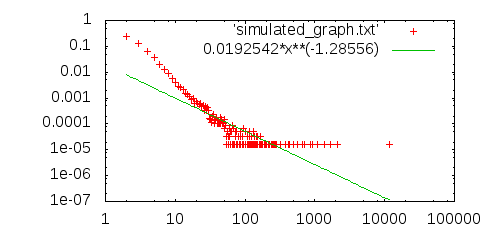
\includegraphics{code/simulated_graph.png}

\chapter{Программа}

Для моделирования веб-графов в соответствии с моделью Боллобаша-Боргса-Риордана-Чайеса был реализован программный продукт, позволяющий считывать реальный ориентированный веб-граф, моделировать графы с различными значениями параметров, сравнивать реальный и модельный графы по распределению степеней вершин и находить те значения параметров, при которых модельный граф наилучшим образом отражает некоторые характеристики реального веб-графа.

\section{Модуль Graph}

Программный модуль Graph позволяет хранить ориентированный граф с заданным количеством вершин и рёбрами между ними, изменять и узнавать количество вершин в графе, добавлять новые вершины и рёбра, узнавать о наличии либо отсутствии ребра между заданными двумя вершинами, а также вычислять показатель одной из важных характеристик графа -- распределения степеней вершин.

Каждый объект графа инкапсулирует целочисленную переменную -- количество вершин в графе, а также множество упорядоченных пар целых чисел. В каждой паре первое число означает номер вершины, из которой выходит ребро графа, а второе число означает номер вершины, в которую входит ребро графа. Все пары образуют множество рёбер графа.

Конструктор по умолчанию создаёт пустой граф, то есть граф, в котором нет ни одной вершины и ни одного ребра, а конструктор копирования полностью копирует ориентированный граф из другого объекта, сохраняя все вершины и рёбра между ними. Деструктор удаляет имеющийся граф.

Функция SetVertexCount принимает в качестве параметра целое число, являющееся новым значением количества вершин графа, и устанавливает в графе данное количество вершин. Функция GetVertexCount позволяет узнать текущее количество вершин графа. Обе функции работают за константное время.

Функция AddEdge принимает в качестве параметров два целых числа -- номера вершин графа, между которыми требуется добавить ребро в граф. Первый параметр -- это номер вершины графа, из которой выходит ребро, а второй параметр -- номер вершины, в которую входит ребро. Вершины нумеруются с нуля. Функция создаёт упорядоченную пару из этих двух чисел и добавляет созданную пару в множество рёбер графа. Функция GetEdge принимает точно такие же параметры и проверяет, имеется ли в графе ребро, выходящее из вершины, номер которой указан в первом параметре, в вершину, номер которой указанан во втором параметре. Для этого функция создаёт упорядоченную пару чисел и ищет её в множестве вершин графа. Если такая пара находится, возвращается истина, иначе -- ложь. Обе функции работают за логарифмическое время от количества рёбер в графе.

Функция EstimateXi оценивает характеристику распределения степеней вершин графа. Степенью вершины считается суммарное количество входящих в вершину рёбер и исходящих из вершины рёбер. Вероятностью встретить вершину заданной степени является отношение количества вершин заданной степени к общему количеству вершин графа. Предполагается, что распределение степеней вершин графа имеет следующий вид:
$$
P = c d^{-\xi},
$$
где $d$ -- степень вершины, $P$ -- вероятность встретить вершину степени $d$ в исследуемом графе, $c$ и $\xi$ -- некие константы, причём $c$ нас интересовать не будет, а вот $\xi$ как раз и является той величиной, которую вычисляет обсуждаемая функция для имеющегося графа. Величина $\xi$ позволяет сравнивать разные графа, то есть выступает в роли некоторой метрики: чем меньше разница между этими величинами у разных графов, тем более похожими мы их будем считать.

Для вычисления степеней всех вершин в фукнции EstimateXi создаётся вектор длиной в количество вершин в графе и заполняется нулями. В каждой ячейке этого вектора будет храниться степень вершины графа (номер ячейки вектора равен номеру вершины графа). После этого перебираются все рёбра графа из множества рёбер графа, у каждого ребра определяются номера вершин, из которой выходит ребро и в которую входит ребро, а потом значения соответствующих ячеек вектора увеличиваются на единицу.

Для вычисления вероятностей встретить вершину с заданной степенью сначала строится отображение из степени вершины графа в количество вершин графа с такой степенью, которое хранится в контейнере map. Мы проходим по всем вершинам графа, для каждой вершины с помощью ранее вычисленного вектора определяет её степень, а дальше проверяем наличие в контейнере map соответствующей пары. Если в контейнере для данной степени уже есть количество таких вершин, то мы просто увеличиваем это количество на единицу, а если такой степени ещё не было в контейнере, то мы добавляет туда новую пару с данной степенью и количеством один. После построения такого отображения мы можем вычислить вероятность встретить вершину с соответствующей степенью.

Поскольку распределение степеней вершин графа $P = c d^{-\xi}$ имеет показательный вид, прологарифмируем его и получим
$$
\ln{P} = \ln{c} - \xi \ln{d}
$$

Полученную прямую можно найти с помощью метода наименьших квадратов, для этого введём следующие обозначения:
$$
y_t = a + b x_t + \epsilon_t
$$
$$
y_t = \ln{P}
$$
$$
a = \ln{c}
$$
$$
b = \xi
$$
$$
x_t = -\ln{d}
$$

По формулам из метода наименьших квадратов
$$
\hat{b} = \frac{Cov(x,y)}{Var(x)} = \frac{\overline{x y}-\overline{x}\overline{y}}{\overline{x^2}-\left(\overline{x}\right)^2}
$$
$$
\hat{a} = \overline{y} - b\overline{x}
$$

При реализации этой формулы в программе не учитываются изолированные вершины, то есть вершины степени нуль, поскольку степени вершин должны быть прологарифмированы, а логарифм нуля не существует. Кроме того вероятность встретить вершину определённой степени может оказаться близкой к нулю и из-за погрешностей вычислений чисел с плавающей точкой не получится вычислить логарифм данного числа. Поэтому вершины такой степени, вероятность встретить которые менее $10^{-9}$ также не учитываются. При вычислении средних значений используется количество учтённых в подсчёте вершин.

Для построения графика зависимости вероятности встретить вершину определённой степени от степеней вершин можно добавить одну строчку в эту функцию, чтобы вывести все точки для графика в файл, а потом построить график, например, с помощью программы gnuplot. Значение константы $c$ можно было бы не вычислять, но для наглядности график можно дополнить прямой, полученной методом наименьших квадратов, поэтому требуется вычислить значение $c$.

Результатом работы данной функции является вычисленное значение константы $\xi$, которое и возвращается.

\section{Модуль RealGraph}

Программный модуль RealGraph позволяет прочитать входные данные реального веб-графа. В данном модуле реализован класс RealGraph, который пронаследован от класса Graph, описанного выше.

Конструктор по умолчанию создаёт пустой граф вызовом конструктора по умолчанию для базового класса, а конструктор копирования полностью копирует ориентированный граф из другого объекта, сохраняя все вершины и рёбра между ними, также с помощью вызова конструктора копирования для базового класса. Деструктор удаляет имеющийся граф.

Функция LoadRealGraph принимает в качестве параметра строку, в которой записано имя входного файла с реальным веб-графом. Входной файл должен быть следующего формата: каждая строка содержит несколько полей, разделённых пробелами. Первые два поля каждой строки -- это префикс хоста и наименование хоста, которые игнорируются данной функцией. В третьем поле содержится идентификатор вершины графа, а все поля, начиная с четвёртого и до конца строки, содержат идентификаторы вершин графа, из которых выходят рёбра, входящие в вершину, указанную в третьм поле строки. Число $-1$ в третьем поле означает внешнюю вершину графа для возможности указания рёбер, идущих из вершин графа наружу или приходящих в граф извне. Подобные строки игнорируются данной функцией.

С помощью простого скрипта на языке Python была вычислена максимальная длина среди всех строк входного файла, а потом был создан буфер в один миллион символов (с запасом), чтобы в него точно поместилась любая строка входного файла.

Файл открывается и читается построчно. Строка записывается в буфер, в ней дважды ищется символ проблема, чтобы пропустить первые два поля, а потом читается число -- идентификатор вершины. Для чтения чисел из строки используется функция strtok из стандартной библиотеки cstring. Если этот идентификатор оказывается равным $-1$, то строка пропускается и мы переходим к обработке следующей строки, иначе читаются все остальные числа до конца строки в цикле.

Все идентификаторы вершин сохраняются в множестве, а рёбра в виде упорядоченных пар идентификаторов вершин -- в векторе. Первым числом пары является идентификатор вершины, из которой выходит ребро (четвёртое поле строки и далее), а вторым числом пары является идентификатор вершины, в которую входит ребро (третье поле строки).

После чтения файла у нас образуется множество различных идентификаторов вершин, которые нам нужно обойти и перенумеровать от $0$ до $N$, где $N$ -- количество вершин графа. Для этого мы создаём контейнер map и для каждого идентификатора записываем в него порядковый номер этого идентификатора при обходе множества итератором.

Теперь остаётся установить количество вершин в графе равным мощности множества различных идентификаторов вершин с помощью вызова функции базового класса, а также пройтись по вектору пар идентификаторов, для каждого индентификатора из пары с помощью отображения узнать его порядковый номер (номер вершины графа) и добавить соответствующее ребро в граф с помощью вызова функции базового класса.

\section{Модуль SimulatedGraph}

Программный модуль SimulatedGraph позволяет соделировать веб-граф по модели Боллобаша-Боргса-Риордана-Чайеса. В данном модуле реализован класс SimulatedGraph, который пронаследован от класса Graph, описанного выше. Класс позволяет устанавливать заданные значения параметров и узнавать установленные значения параметров, выбирать вершины обеими описанными в модели способами и генерировать граф для любого заданного значения параметра времени генерации.

Каждый объект графа инкапсулирует параметры модели $\alpha, \beta, \gamma, \delta_{in}, \delta_{out}$, а также векторы in\_numerator и out\_numerator для хранения значения числителей вероятностей для выбора соответствующих вершин при моделировании.

Конструктор по умолчанию создаёт пустой граф вызовом конструктора по умолчанию для базового класса, и заполняет параметры модели значениями по умолчанию, а конструктор копирования полностью копирует ориентированный граф из другого объекта, сохраняя все вершины и рёбра между ними, также с помощью вызова конструктора копирования для базового класса, и копирует установленные параметры модели. Деструктор удаляет имеющийся граф.

Функции SetAlpha, SetBeta и SetDeltaIn принимают в качестве параметра дробное число и устанавливают значение $\alpha$, $\beta$ и $\delta_{in}$ соответственно равным заданному числу. Поскольку $\gamma = 1 - \alpha - \beta$ и $\delta_{out} = 0$, то эти значения устанавливаются автоматически, а $\gamma$ автоматически пересчитывается при установке нового значения $\alpha$ и/или нового значения $\beta$.

Функции GetAlpha, GetBeta, GetGamma, GetDeltaIn, GetDeltaOut возвращают текущее установленное значение параметра $\alpha$, $\beta$, $\gamma$, $\delta_{in}$ и $\delta_{out}$ соответственно.

Функция ChooseVertexAccordingToIn выбирает одну из вершин графа по описанному в модели принципу. В нулевой ячейке вектора in\_numerator хранится значение числителя вероятности, с которой следует выбрать нулевую вершину, а в произвольной $i$-ой ячейке хранится сумма числителей вероятностей, с которыми следует выбрать вершины от нулевой до $i$-ой включительно. Поэтому в последней ячейке этого вектора по сути хранится число, которое можно считать длиной некоторого отрезка, на который требуется кинуть случайную точку, а потом узнать, в какой ячейке записано минимальное число, больше выпавшего случайной точкой. Функция использует генератор псевдослучайных чисел для получения случайного числа у нужном диапазоне, а далее с помощью алгортма upper\_bound находит нужную вершину (для корректной работы этой функции значение последней ячейки вектора временно увеличивается на 1, а потом возвращается обратно).

Функция ChooseVertexAccordingToOut работает аналогично функции ChooseVertexAccordingToIn, только работает с вектором out\_numerator.

Функция GenerateGraph получает в качестве параметра время генерации модельного графа, а затем моделирует граф по модели Боллобаша-Боргса-Риордана-Чайеса.

Сначала функция очищает векторы in\_numerator и out\_numerator и создаёт граф, состоящий из одной вершины с петлёй, а также записывает в векторы начальные значение вероятностей $1 + \delta_{in}$ и $1 + \delta_{out}$.

Далее функция выполняет цикл заданное в параметре функции время. На каждой итерации определяется псевдослучайное число от 0 до 1 включительно. Дальше резулируется один из трёх случаев: с вероятностью $\alpha$ выбирается вершина функцией ChooseVertexAccordingToIn, добавляется новая вершина в граф и новое ребро из добавленной вершины в выбранную, с вероятностью $\beta$ выбираются две вершины графа (первая функцией ChooseVertexAccordingToOut, вторая функцией ChooseVertexAccordingToIn) и проводится ребро из первой во вторую, с вероятностью $\gamma$ выбирается вершина графа функцией ChooseVertexAccordingToOut, добавляется новая вершина в граф и проводится ребро из выбранной вершины в добавленную. В каждом из трёх случаев векторы in\_numerator и out\_numerator изменяются в соответствии с добавленными вершинами и рёбрами (для новой вершины добавляется ячейка в вектор с начальным значением вероятности, после добавления ребра во все ячейки нужного вектора, начиная с номера вершины, у которой добавилось ребро, все значения увеличиваются на единицу, потому что поменялась степень вершины, а значит и кумулятивные суммы).

Полученный в результате граф может быть оценён функцией базового класса EstimateXi для сравнения с реальным графом.

\section{Модуль Main}

Программный модуль Main предназначен для подбора наилучших значений параметров модели Боллобаша-Боргса-Риордана-Чайеса. В начале модуля задаются константные массивы перебираемых значений параметров, а также некоторые важные константы (время генерирования модельного графа, начальная инициализация генератора датчика псевдослучайных чисел, количество повторений моделирования графа с одними и теми же параметрами, точность вычислений значений параметров с плавающей точкой).

Функция main инициализирует датчик псевдослучайных чисел, создаёт объект реального графа и функцией LoadRealGraph загружает граф из входного файла, затем функцией EstimateXi оценивает показатель степенного распределения вероятностей степеней вершин и выводит это значение в стандартный поток вывода. После этого инициализируются значения переменных для наилучших значений параметров и в циклах перебираются все возможные сочетания параметров модели с учётом условия $\alpha + \beta < 1 - \epsilon$.

На каждой итерации внутреннего цикла создаётся объект модельного графа, функциями SetAlpha, SetBeta и SetDeltaIn устанавливаются текущие значения параметров, а затем функцией GenerateGraph моделируется граф. Затем у полученного графа функцией EstimateXi вычисляется показатель степенного распределения степеней вершин. Все эти действия повторяются заданное количество раз, а потом вычисляется математическое ожидание и дисперсия величины $\xi$, чтобы она меньше зависела от случайностей. Если полученное среднее значение $\xi$ оказалось лучше ранее найденного, то текущие параметры модели сохраняются в качестве наилучших, а также выводится информация о текущих результатах в стандартный поток вывода.

В конце выводится информация о наилучших значениях параметров в стандартный поток вывода, а также информация о том, насколько сильно $\xi$ для реального графа отличается от этой же величины для смоделированного графа при полученных наилучших параметрах.

\chapter{Выводы}
We worked hard, and achieved very little.

\bibliographystyle{abbrv}
\begin{thebibliography}{9}

\bibitem{}
Степанов В. Е. О вероятности связности случайного графа $g_m(t)$ // Теория вероятностей и ее применения. 1970. Т. 15. № 1. С. 55–67.
\bibitem{}
Степанов В. Е. Фазовый переход в случайных графах // Теория вероятностей и ее применения. 1970. Т. 15. № 2. С. 187–203.
\bibitem{}
Степанов В. Е. Структура случайных графов $g_n(x|h)$ // Теория вероятностей и ее применения. 1972. Т. 17. № 3. С. 227–242.
\bibitem{}
Колчин В. Ф. Случайные графы. М.: Физматлит, 2004.
\bibitem{}
Bollobas B. Random Graphs. Cambridge: Cambridge Univ. Press, 2001.
\bibitem{}
Алон Н., Спенсер Дж. Вероятностный метод. М: Бином. Лаборатория знаний, 2007.
\bibitem{}
Janson S., Luczak T., Rucinski A. Random graphs. N.Y.: Wiley, 2000.
\bibitem{}
Маргулис Г. А. Вероятностные характеристики графов с большой связностью // Проблемы передачи информации. 1974. Т. 10. С. 101–108.
\bibitem{}
Karp R. The transitive closure of a random digraph // Random structures and algorithms. 1990. V. 1. P. 73–94.
\bibitem{}
Карлин С. Основы теории случайных процессов. М: Мир, 1971.
\bibitem{}
Barabasi L.-A., Albert R. Emergence of scaling in random networks // Science. 1999. V. 286. P. 509–512.
\bibitem{}
Barabasi L.-A., Albert R., Jeong H. Scale-free characteristics of random networks: the topology of the world-wide web // Physica A. 2000. V. 281. P. 69–77.
\bibitem{}
Albert R., Jeong H., Barabasi L. A. Diameter of the world-wide web // Nature. 1999. V. 401. P. 130–131.
\bibitem{}
Bollobas B., Riordan O. Mathematical results on scale-free random graphs. Handbook of graphs and networks. Weinheim: Wiley-VCH. 2003. P. 1–34.
\bibitem{}
Райгородский А. М. Экстремальные задачи теории графов и анализ данных. М.–Ижевск: НИЦ «РХД», 2009.
\bibitem{}
Stoimenow A. Enumeration of chord diagrams and an upper bound for Vassiliev invariants // J. Knot Theory Ramifications. 1998. V. 7. N. 1. P. 93–114.
\bibitem{}
Bollobas B., Riordan O. The diameter of a scale-free random graph // Combinatorica. 2004. V. 24. N. 1. P. 5–34.
\bibitem{}
Bollobas B., Riordan O., Spencer J., Tusnady G. The degree sequence of a scale-free random graph process // Random Structures Algorithms. 2001. V. 18. N. 3. P. 279–290.
\bibitem{}
Kumar R., Raghavan P., Rajagopalan S., Sivakumar D., Tomkins A., Upfal E. Stochastic models for the web graph // Proc. 41st Symposium on Foundations of Computer Science. 2000.

\end{thebibliography}
\newpage

\begin{appendices}
\chapter{Исходный код программы}
{\footnotesize
\lstinputlisting{code/plot.gnu}
\newpage
\lstinputlisting{code/max_line_length.py}
\newpage
\lstinputlisting{code/graph.h}
\newpage
\lstinputlisting{code/graph.cpp}
\newpage
\lstinputlisting{code/simulated_graph.h}
\newpage
\lstinputlisting{code/simulated_graph.cpp}
\newpage
\lstinputlisting{code/real_graph.h}
\newpage
\lstinputlisting{code/real_graph.cpp}
\newpage
\lstinputlisting{code/main.cpp}
}

\chapter{Результат работы программы}
{\footnotesize
\lstinputlisting{code/output.txt}
}
\end{appendices}

\end{document}
